\section{Durchführung}
\label{sec:Durchführung}

\subsection{Untersuchung der Moden mit einem Oszilloskop}
\subsubsection{Aufbau}
Der Aufbau ist in Abbildung \ref{fig:moden_aufbau} zu sehen.
Das Reflexklytron wird an die Spannungquelle angeschlossen und die Refelktorspannung wird rechteck moduliert.
Die ausgestrahlten Mikrowellen werden durch einen Hohleieter zu einem Einwegleiter gesendet.
Der Einwegleiter sorgt dafür, dass keine Mikrowellen zurück in das Reflexklytron gelangen.
Danach folgt ein Frequenzmessgerät mit dem die Frequenz der Moden bestimmt wird.
Auf dieses folgt ein Attunator und ein Detektor, der an ein Oszilloskop angeschlossen wird.

\begin{figure}
    \centering
    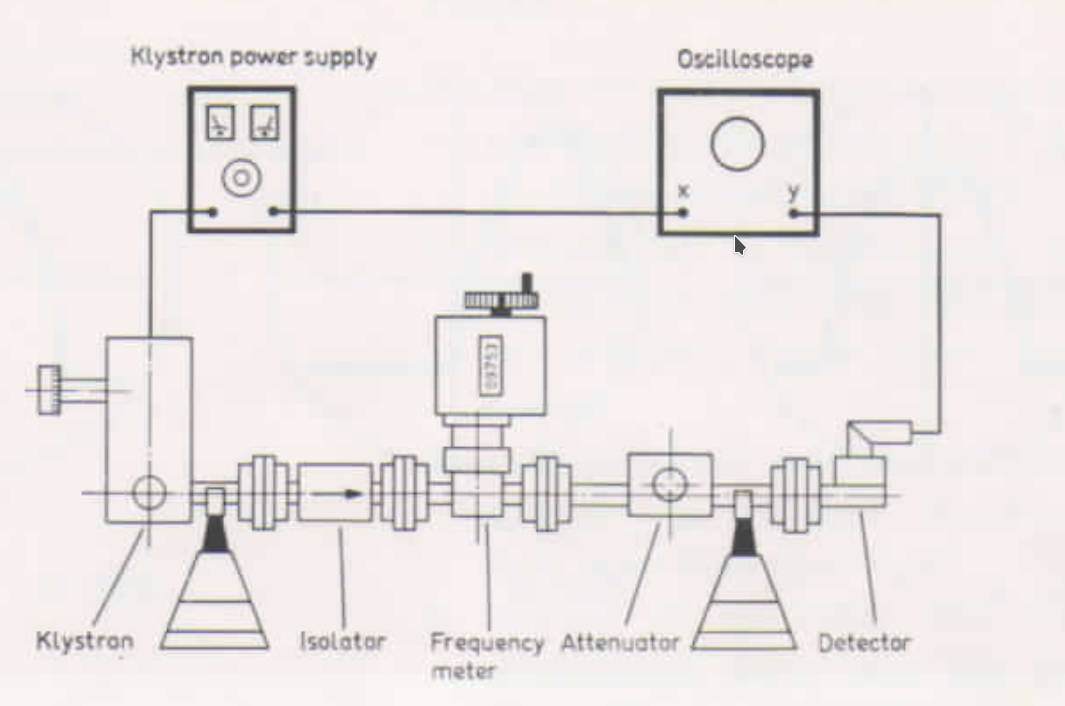
\includegraphics[width=0.75\textwidth]{content/data/Aufbau_Moden.png}
    \caption{Aufbau zur Bestimmung der Schwingungsmoden des Reflexklytron. Bild entnommen aus \cite[8]{Anleitung}.}
    \label{fig:moden_aufbau}
\end{figure}

\subsubsection{Messung der Moden}
\label{sec:moden_durchfuehrung}
Das Reflexklytron sollte nun Mikrowellen ausstrahlen und die Refelktorspannung muss Rechteck moduliert sein. Das Dämpfugsglied wird auf $\SI{30}{\dB}$ gestellt.
Nun sollte auf dem Oszilloskop eine parabelförmige Modenkurve sichtbar sein.
Mit dem Frequenzmessgerät wird nun die Frequenz der Mode bestimmt indem die Frequenz am Messgerät so eingestellt wird, dasss am Hochpunkt der Mode ein 'Dip' zu sehen ist.
Der 'Dip' entsteht durch die Messung der Frequenz mit dem Messgerät.
Die Frequenz die dann am Messgerät eingestellt ist wird notiert.
Nun wird das Frequenzmessgerät verstimmt und die Maximale Spannung der Mode vom Oszilloskop abgelesen.
Danach wird die Refelktorspannung verändert bis die Spannung zum Anfang der Mode und zum Ende der Mode vom Oszilloskop abgelesen werden kann.
Der Ablauf wird für zwei weitere Refelktorspannungen wiederholt.


Nun wird die höchste Mode gesucht.
Von dieser wird die halbe maximale Amplituden Leistung vermessen.
Dies geschieht indem zunächst das Frequenzmessgerät auf $\SI{9000}{\mega\Hz}$ eingestellt wird.
Darauf wird die Refelktorspannung so lange variiert bis sich der 'Dip' auf halber Amplituden Höhe befindet.
Dadurch lässt sich die breite der Kurve bestimmen und so die Abstimm-Empfindlichkeit $\frac{f_0 - f_1}{U_0 - U_1}$.

\subsection{Messung der Frequenz, Wellenlänge und Dämpfung im Hohleieter}
\subsubsection{Aufabu}
\label{sec:aufbau}
Aus dem Aufbau in Abbildung \ref{fig:moden_aufbau} wird nun der Detektor für das Oszilloskop entfernt.
Anstelle dessen wird ein Stehwellendetektor eingebaut, der an das SWR-Meter angeschlossen ist.
Hinter dem Stehwellendetektor wird ein Kurzschluss oder ein Abschluss eingebaut.
Zunächst wird der Abschluss verwendet.
Das Dämpfungsglied wird auf $\SI{20}{\dB}$ eingestellt.
Am SWR-Meter wird der $\SI{40}{\dB}$ Knopf gedrückt und eine Bandbreite von $\SI{20}{\Hz}$ eingestellt.
Das Refelktorspannung des Klystrons liegt bei ungefähr$ \SI{200}{\V}$ und wird rechteckmoduliert.
Am SWR-Meter sollte ein Maximum zu sehen sein.

\subsubsection{Frequenzmessung}
Am Frequenzmessgerät wird die Frequenz eingestellt die den minimalen Ausschlag am SWR-Meter erzeugt.
Diese Frequenz wird notiert.

\subsubsection{Wellenlängenmessung}
Der Abschluss wird durch den Kurzschluss ersetzt.
Der Stehwellendetektor wird an einen Ort minimalen Ausschlags des SWR-Meter verschoben.
Die Position der Stehwellendetektor wird notiert.
Nun wird der Detektor ins nächste Minimum verschoben und die Position wird erneut notiert.
Die Wellenlänge ergibt sich nun aus der doppelten Distanz zwischen den beiden Minima.
Aus der Wellenlänge kann nun nach Gleichung \ref{eq:wellenlaenge_hohleiter} die Frequenz bestimmt werden.

\subsubsection{Dämpfungsmessung}
\subsubsection{Leistungsverhältnis Methode}
Der Kurzschluss wird wieder durch den Abschluss ersetzt.
Das Klystron wird auf $\SI{9000}{\Hz}$ eingestellt.
Die Dämpfung wird nun so eingstellt, das am SWR-Meter ein vollauschlag zu sehen ist.
Die Einstellung des Dämpfungsglieds wird notiert.
Die Dämpfung wird nun in $\SI{2}{\dB}$ Schritten der unteren Skala des SWR-Meters erhöht.
Die Dämpfung jeden Schritts wird dabei am Dämpfungsglied abgelesen.
Die Dämpfung wird bis auf $\SI{10}{\dB}$ erhöht.

\subsection{Stehwellenmessung}
\subsubsection{Aufbau}
Der Aufbau wird wie zuvor in Abschnitt \ref{sec:aufbau} beschrieben, übernommen.
Allerdings wird zwischen dem Abschluss und dem Stehwellendetektor ein Gleitschraubentransformator eingebaut.
Das Dämpfungsglied steht auf $\SI{20}{\dB}$.
Die Schraube des Gleitschraubentransformator sollte zu Anfang der Messung ganz heraus geschraubt sein.
Es sollte darauf geachtet werden, dass vor der Messung beim Bewegen des Stehwellendetektor sich der Auschlag am SWR-Meter nur wenig verändert.

\subsubsection{Messung durch direkte Methode}
Die Schraubentiefe des Gleitschraubentransformator wird auf $\SI{5}{\milli\meter}$ eingestellt.
Der Stehwellendetektor wird in ein Maximum verschoben.
Die Verstärkung des SWR-Meter muss nun so eingestellt werden, dass dieses $1$ anzeigt.
Jetzt wird der Stehwellendetektor in ein Minimum verschoben und der Wert am SWR-Meter wird abgelesen.
Dieser Ablauf wird für Schraubentiefen von $3,7 \; \text{und} \; 9 \, \si{\milli\meter}$ wiederholt.
\\\\
Diese Methode funktioniert allerdings nicht für große Welligkeiten, dafür werden andere Methoden benötigt.
\subsubsection{3 dB-Methode}
Die Schraube des Gleitschraubentransformator wird auf $\SI{9}{\milli\meter}$ gestellt.
Der Stehwellendetektor wird in ein Minimum verschoben und die Verstärkung des SWR-Meter wird so eingestellt, dass dies $\SI{3}{\dB}$ anzeigt.
Die Sonde des Stehwellendetektors wird nun so verschoben, dass das SWR-Meter einen Wert von $\SI{0}{\dB}$ anzeigt, dann wird die Position des Schlittens notiert.
Nun wird der Schlitten in die andere Richtung verschoben bis wiederrum ein Wert von $\SI{0}{\dB}$ angezeigt wird.
Danach wird der Abschluss durch einen Kurzschluss ersetzt und der Abstand zwischen zwei Minimas wird bestimmt um die Wellenlänge im Hohleiter zu bestimmen.
Das SWR kann nun nach 
\begin{equation}
    S \approx \frac{\lambda _\text{g}}{\pi \left ( d_1 - d_2 \right )}
    \label{eq:3db_SWR}
\end{equation}
berechnet werden.

\subsubsection{Abschwächer Methode}
\label{sec:abschwaecher_methode}
Die Schraube des Gleitschraubentransformator steht nun wieder auf $\SI{9}{\milli \meter}$.
Der Detektor wird in ein Minimum verschoben.
Jetzt wird das Dämpfungsglied auf $A_1 = \SI{20}{\dB}$ eingestellt und die Verstärkung des SWR-Meters wird so eingestellt, dass dies $\SI{3}{\dB}$ anzeigt.
Nun wird der Detektor in ein Minima verschoben und währendessen die Dämpfung so varriert, dass das SWR-Meter weiterhin $\SI{3}{\dB}$ anzeigt.
Nun wird die Dämpfung $A_2$ am Dämpfungsglied abgelesen und notiert.
Das Stehwellenverhältnis ergibt sich nun aus 
\begin{equation}
    S = 10^{\frac{A_2 -A_1}{20}}
    \label{eq:daempfung_SWR}
\end{equation}